\section{Participant 2}

% JC

\subsection{Date \& Time}
\begin{table}[ht]
  \begin{tabular}{|P{3cm}|P{3cm}|}
	\multicolumn{2}{c}{\textbf{2016-08-03}}    	\\ \hline
    Start Time      			& End Time   					\\ \hline
   \textbf{12:23:50} 	& \textbf{12:42:23}    	\\ \hline
   \multicolumn{2}{c}{Duration}    						\\ \hline
   \multicolumn{2}{c}{\textbf{00:18:33}} 			\\ \hline
  \end{tabular}
  \newline\newline
  \caption{P2: Date and Time}\label{dandt2}
\end{table}

\subsection{Questions}
\begin{itemize} 
  \item[\XSolidBrush] Are you a Student?
  \item[\Checkmark] Did you work in a team?
  \item[\Checkmark] Did you listen to music?
  \item[\XSolidBrush] Did you feel tired?
  \item[\Checkmark] Did you enjoy the tasks?
  \item[\Checkmark] Did you give all you attention to the tasks?
  \item[\XSolidBrush] Were you distracted during the tasks?
  \item[\XSolidBrush] Did you feel stressed
  \item[\Checkmark] Do you think the tasks were easy?  
\end{itemize}


\FloatBarrier
\newpage
\subsection{Accelerometer}

\begin{figure}[ht]
	\centering
	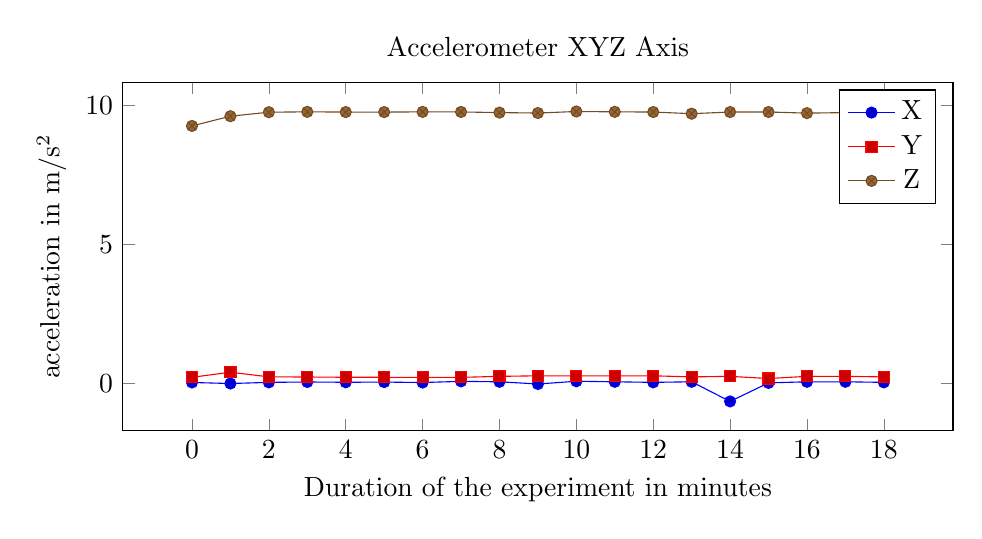
\begin{tikzpicture}
\begin{axis}[
	height=6cm,
	width=\textwidth,
	xlabel=Duration of the experiment in minutes,
	ylabel=acceleration in m/s$^2$,
	title=Accelerometer XYZ Axis,
	unbounded coords=discard],
	
%X
\addplot coordinates {
(0 , 0.0349651822609)
(1 , -0.00309673126316)
(2 , 0.0382930208571)
(3 , 0.0523034957619)
(4 , 0.0420292439048)
(5 , 0.049033425)
(6 , 0.0326879590952)
(7 , 0.0751864109167)
(8 , 0.05883789)
(9 , -0.019607544)
(10 , 0.07846069)
(11 , 0.05883789)
(12 , 0.039230347)
(13 , 0.05883789)
(14 , -0.64723206)
(15 , 0.019607544)
(16 , 0.05883789)
(17 , 0.05883789)
(18 , 0.039230347)
};

%Y
\addplot coordinates {
(0 , 0.220863674783)
(1 , 0.403620667895)
(2 , 0.23722984381)
(3 , 0.231626238095)
(4 , 0.222285678571)
(5 , 0.221095690909)
(6 , 0.217615762857)
(7 , 0.219015755833)
(8 , 0.25497437)
(9 , 0.2745819)
(10 , 0.2745819)
(11 , 0.2745819)
(12 , 0.2745819)
(13 , 0.23536682)
(14 , 0.25497437)
(15 , 0.17651367)
(16 , 0.25497437)
(17 , 0.25497437)
(18 , 0.23536682)
};

%Z
\addplot coordinates {
(0 , 9.26770895652)
(1 , 9.61774347368)
(2 , 9.76181833333)
(3 , 9.77489447619)
(4 , 9.76648904762)
(5 , 9.76563831818)
(6 , 9.77396304762)
(7 , 9.77069233333)
(8 , 9.74780316161)
(9 , 9.73178425312)
(10 , 9.78743477033)
(11 , 9.77489304762)
(12 , 9.76742633556)
(13 , 9.70858834222)
(14 , 9.76742655645)
(15 , 9.76935722354)
(16 , 9.72819595862)
(17 , 9.74780318532)
(18 , 9.70858858813)
};

\addlegendentry{X}
\addlegendentry{Y}
\addlegendentry{Z}
\end{axis}
\end{tikzpicture}
 	\vspace{5 mm}
\end{figure}

\FloatBarrier
\subsection{Light Level}
\begin{figure}[ht]
	\centering
	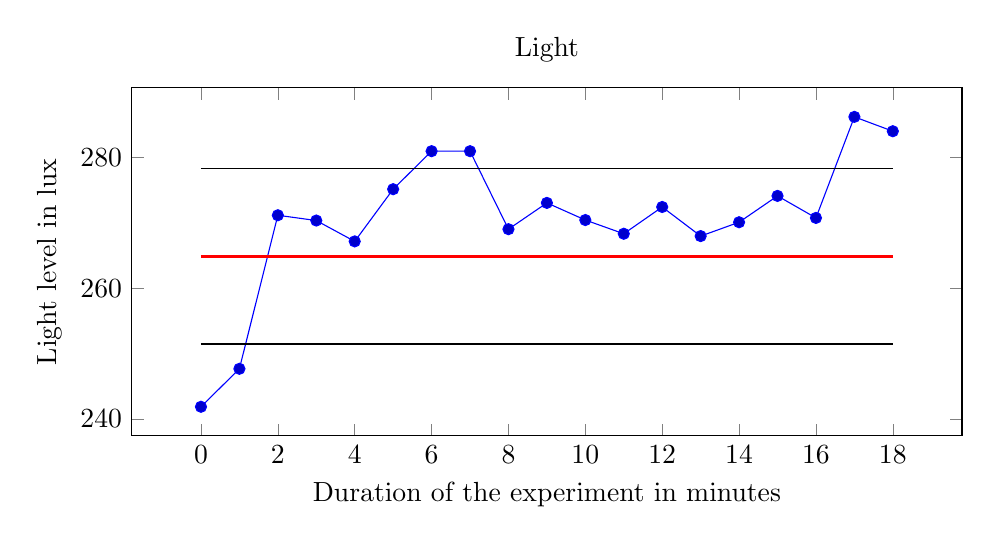
\begin{tikzpicture}
\begin{axis}[
	height=6cm,
	width=\textwidth,
	xlabel=Duration of the experiment in minutes,
	ylabel=Light level in lux,
	title=Light,
	unbounded coords=discard],
	
\addplot coordinates {
(0 , 241.869565217)
(1 , 247.684210526)
(2 , 271.19047619)
(3 , 270.380952381)
(4 , 267.19047619)
(5 , 275.181818182)
(6 , 281.0)
(7 , 281.0)
(8 , 269.056565454)
(9 , 273.082245)
(10 , 270.457685359)
(11 , 268.358045125)
(12 , 272.456782138)
(13 , 268.0)
(14 , 270.121246868)
(15 , 274.154865478)
(16 , 270.782398425)
(17 , 286.252546845)
(18 , 284.054086785)
};

\addplot[mark=none, red, very thick] coordinates {(0, 264.928214098) (18, 264.928214098)};

\addplot[mark=none, black] coordinates {(0, 251.47691699) (18, 251.47691699)};
\addplot[mark=none, black] coordinates {(0, 278.379511206) (18, 278.379511206)};

\end{axis}
\end{tikzpicture}
 	\vspace{5 mm}
\end{figure}

\newpage
\FloatBarrier
\newpage
\subsection{Noise Level}
\begin{figure}[ht]
	\centering
	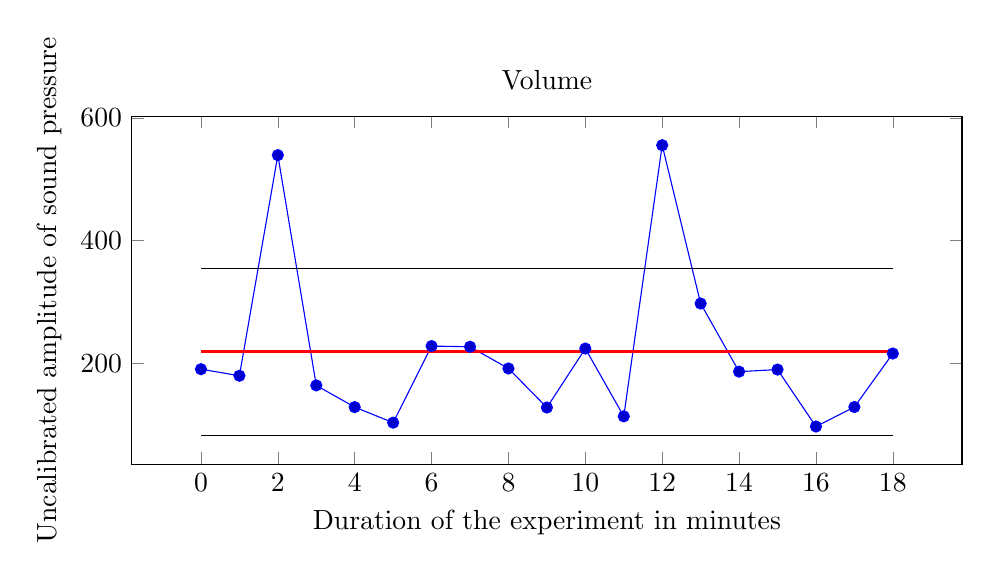
\begin{tikzpicture}
\begin{axis}[
	height=6cm,
	width=\textwidth,
	ylabel=Uncalibrated amplitude of sound pressure,
	xlabel=Duration of the experiment in minutes,
	title=Volume,
	unbounded coords=discard],

\addplot coordinates {
(0 , 190.434782609)
(1 , 179.736842105)
(2 , 539.238095238)
(3 , 164.0)
(4 , 128.619047619)
(5 , 103.318181818)
(6 , 228.095238095)
(7 , 227.0)
(8 , 191.596186522)
(9 , 127.958334583)
(10 , 224.056548712)
(11 , 113.580190875)
(12 , 555.4568753253)
(13 , 297.4565454254)
(14 , 186.4298341674)
(15 , 189.8012096456)
(16 , 97.0)
(17 , 128.8121400108)
(18 , 215.9958225684)
};

\addplot[mark=none, red, very thick] coordinates {(0, 219.063169641) (18, 219.063169641)};

\addplot[mark=none, black] coordinates {(0, 83.0123913636) (18, 83.0123913636)};
\addplot[mark=none, black] coordinates {(0, 355.113947918) (18, 355.113947918)};

\end{axis}
\end{tikzpicture}
 	\vspace{5 mm}
\end{figure}

\FloatBarrier

\subsection{Location}
minute 0 : -3.6881917, 40.4579957
minute 1 : -3.68815341053, 40.4579801474)
from minute 2 : -3.6881432, 40.457976)

Madrid, Spain 

\FloatBarrier